

Se produjo el diagrama de Gantt acorde a la tabla recién mostrada, y se marcó el camino crítico en rojo.
\begin{figure}[H]
	\centering
	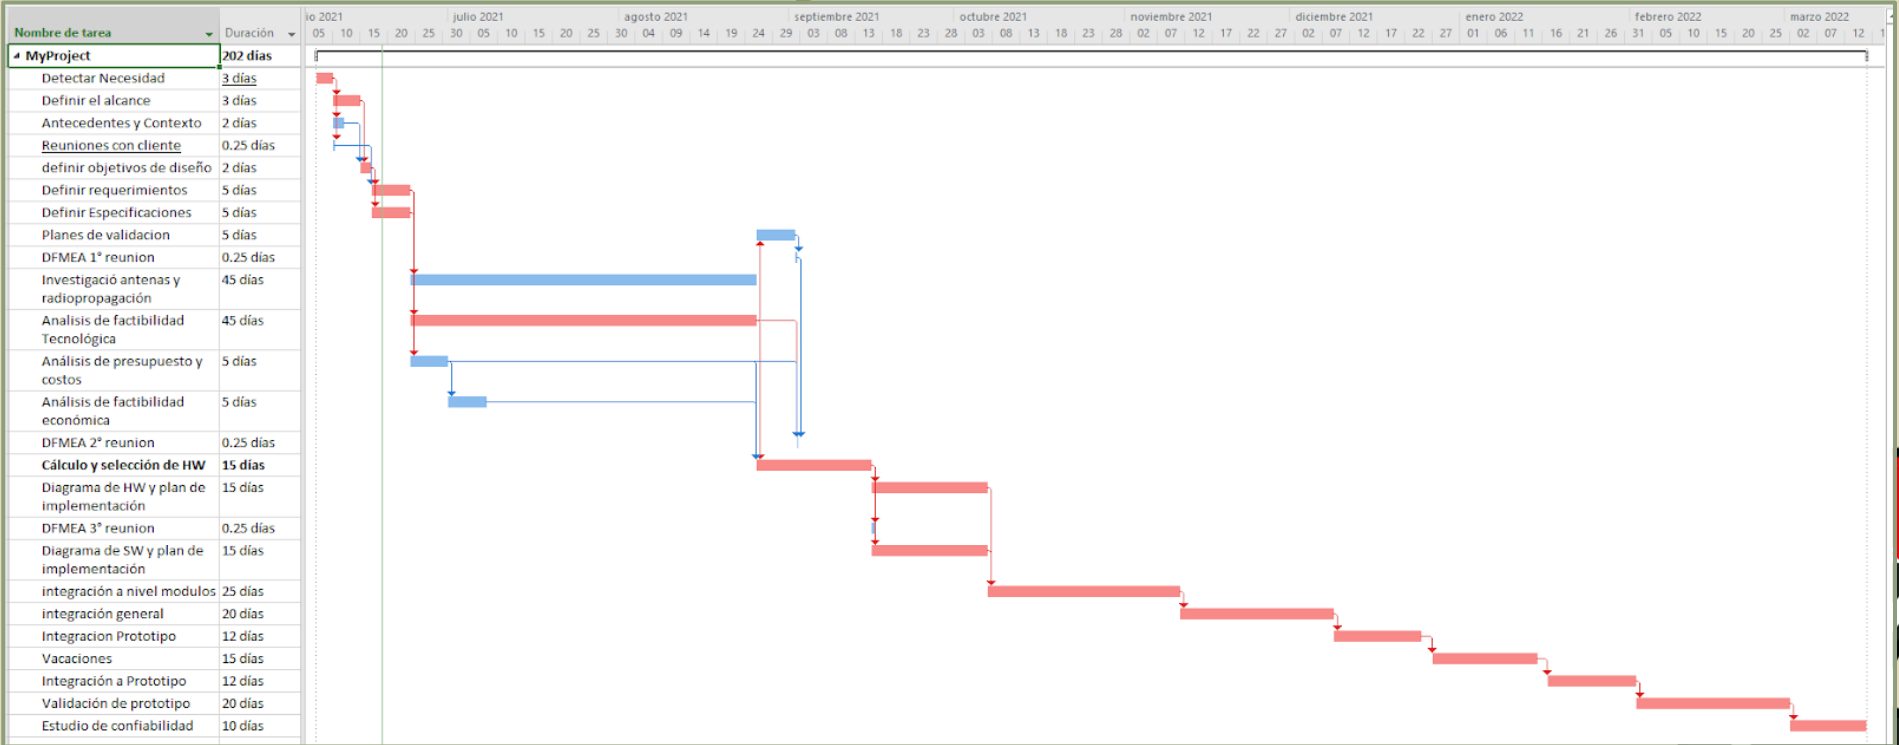
\includegraphics[width=1\linewidth]{ImagenesFactibilidad/project}
	\label{fig:gantt}
	\caption{Diagrama de Gantt del proyecto.}
\end{figure}

Luego se realizó una simulación de montecarlo utilizando la distribución $\beta$ para las variables aleatorias, obteniendo el siguiente gráfico donde se ve la probabilidad de terminar el proyecto en un intervalo de $1461 \ \sim \ 1937 $ horas con una probabilidad del 95$\%$
\begin{figure}[H]
	\centering
	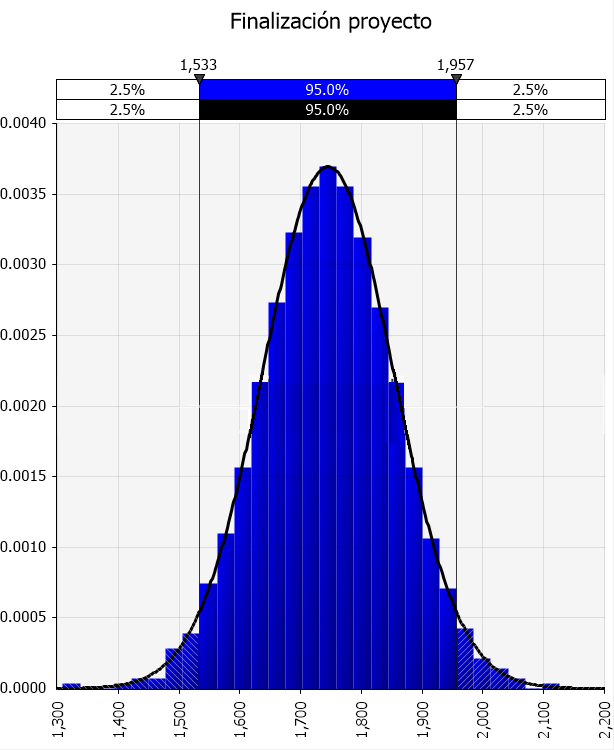
\includegraphics[width=0.5\linewidth]{ImagenesFactibilidad/montecarlo}
	\label{fig:montecarlo_tiempos}
	\caption{Simulación de montecarlo.}
\end{figure}

Esta distribución es el lapso de tiempo entre que se comienza el proyecto y se termina, a travez del camino crítico. 
La cantidad de horas de ingeniería por ingeniero se muestran a continuación, teniendo en cuenta la paralelización de actividades y que se dispone de 4 trabajadores.
\begin{figure}[H]
	\centering
	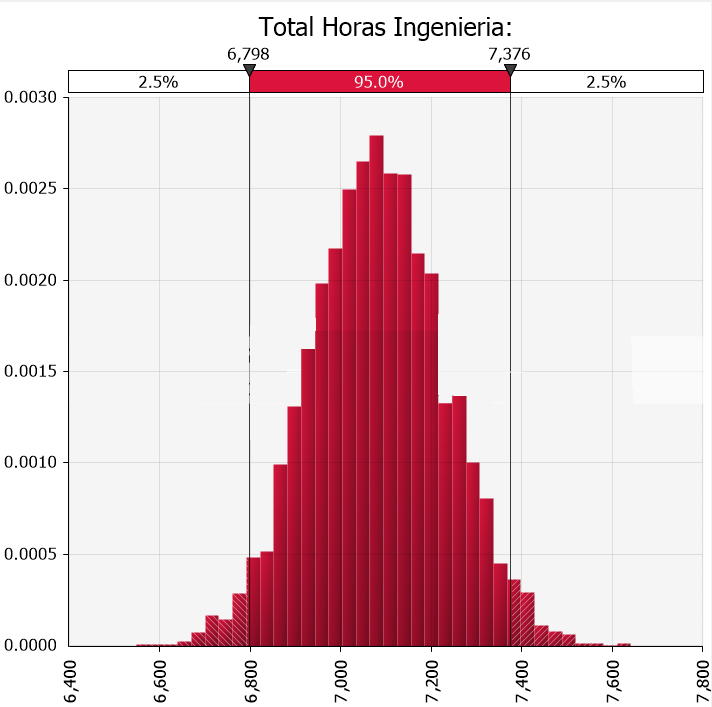
\includegraphics[width=0.5\linewidth]{ImagenesFactibilidad/montecarlo_tiempo_largo}
	\label{fig:montecarlo_tiempos_ing}
	\caption{Simulación de montecarlo para tiempo de ingeniería.}
\end{figure}
Se puede observar que el timepo total de horas de ingeniería corresponde a un rango entre aproximadamente 6800 $\sim$ 7400 horas.